% CAS 2026 (International Semiconductor Conference, Sinaia) - IEEE format
\documentclass[conference]{IEEEtran}

\usepackage{graphicx}
\usepackage{booktabs}
\usepackage{amsmath}
\usepackage{cite}

\graphicspath{{../figures/}}

\begin{document}

\title{Fully Integer-Quantized Thermal Image Super-Resolution\\
on Sub-Dollar Microcontrollers}

\author{
\IEEEauthorblockN{Adrian-Gabriel Diaconu}
\IEEEauthorblockA{\textit{TODO: affiliation}\\
TODO: email}
% TODO: co-authors / advisor
}

\maketitle

\begin{abstract}
% TODO (write last). Skeleton:
% - Low-cost thermal sensors (e.g. MLX90640) output 32x24 px frames.
% - We deploy x2 CNN super-resolution fully on-device on ESP32 and RP2040.
% - Contribution 1: INT8-friendly architecture modifications enabling
%   FULL-integer quantization (int8 activations AND weights, int8 I/O) for
%   five compact SR networks -- no hybrid ops, mandatory for esp-nn/TFLM.
% - Contribution 2: cross-board benchmark: latency, memory, flash, quality,
%   estimated energy; quantization PSNR drop < X dB.
\end{abstract}

\begin{IEEEkeywords}
super-resolution, thermal imaging, quantization, TinyML, microcontrollers,
TensorFlow Lite Micro
\end{IEEEkeywords}

\section{Introduction}
% TODO:
% - Motivation: MLX90640-class sensors are cheap but 32x24; SR raises utility
%   (presence detection, HMI) without better optics/sensor cost.
% - Constraint: MCU deployment needs full-integer INT8; partial (hybrid)
%   quantization is REJECTED by ESP32 TFLM (esp-nn) at runtime.
% - Contributions list (method + benchmark).

\section{Related Work}
% TODO:
% - Compact SISR: SRCNN, ESPCN \cite{shi2016espcn}, FSRCNN \cite{dong2016fsrcnn},
%   EDSR \cite{lim2017edsr}.
% - TinyML inference: TFLite Micro \cite{david2021tflm}.
% - Thermal SR at very low resolution; MLX90640 dataset \cite{zhu2021thermal}.
% - FLIR-IISR dataset (TODO: citation).

\section{Method: Full-INT8 SR Networks}
\subsection{INT8-friendly architecture modifications}
% TODO: Table of op substitutions and why:
% - Tanh -> ReLU (ESPCN): single activation type, cheap int8 kernel.
% - PReLU -> ReLU (FSRCNN): PReLU has no efficient TFLM int8 path.
% - ConvTranspose 9x9 s2 -> Conv 3x3 + depth_to_space (FSRCNN-ds).
% - EDSR residual scaling (0.1) folded into conv weights post-training ->
%   deployed graph is pure Conv2D/Add.
% - Resulting op vocabulary: CONV_2D, (ADD,) DEPTH_TO_SPACE. int8 I/O.
\subsection{Training and quantization pipeline}
% TODO: Keras end-to-end (train-what-you-flash), PTQ with representative
% dataset, int8 I/O; contrast with the PyTorch->ONNX->TF hybrid pipeline
% failure mode (dynamic-range quantization rejected on-device).

\section{Experimental Setup}
\subsection{Dataset and protocol}
% TODO: FLIR-derived pairs: 1238/219 train/val, grayscale, whole-frame resize
% to 64x48 (HR), x2 downsample to 32x24 (LR); justify whole-frame FOV
% statistics vs MLX90640. MLX90640 frames: qualitative only (native 32x24,
% no ground truth exists at 64x48).
\subsection{Hardware platforms}
% TODO: ESP32-DevKitC V4 (no PSRAM), 240 MHz dual-core Xtensa LX6, ~520 KB
% SRAM (fragmented heap constraint); Raspberry Pi Pico, RP2040 @ 133 MHz
% Cortex-M0+, 264 KB SRAM. TFLM runtimes: esp-nn / pico-tflmicro.
% Energy: ESTIMATED chip-level datasheet currents x measured latency
% (TODO: exact datasheet values + citations).

\section{Results}
\subsection{Quality and quantization drop}
% TODO: pull from results/main_table.csv
\begin{table}[t]
\caption{Models, footprint and reconstruction quality (val split).}
\label{tab:quality}
\centering
\begin{tabular}{lrrrrr}
\toprule
Model & Params & kMAC & Flash & PSNR$_{f32}$ & $\Delta$PSNR$_{int8}$ \\
      &        &      & (KB)  & (dB)         & (dB) \\
\midrule
% TODO rows from main_table.csv
\bottomrule
\end{tabular}
\end{table}

\subsection{On-device performance}
\begin{table}[t]
\caption{On-device latency, memory and estimated energy.}
\label{tab:board}
\centering
\begin{tabular}{lrrrrr}
\toprule
Model & \multicolumn{2}{c}{ESP32} & \multicolumn{2}{c}{Pico} & \\
 & ms & KB arena & ms & KB arena & est.\ mJ \\
\midrule
% TODO rows from main_table.csv; EDSR-Tiny expected "n/f" on ESP32
\bottomrule
\end{tabular}
\end{table}

\begin{figure}[t]
\centering
% 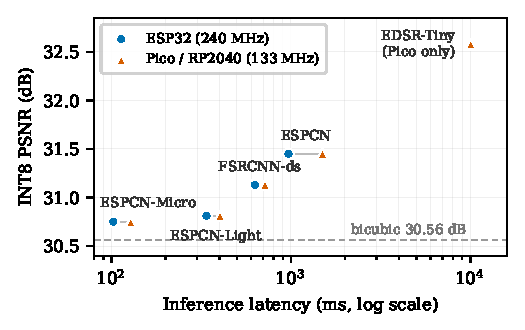
\includegraphics[width=\columnwidth]{psnr_vs_latency.pdf}
\caption{Quality--latency trade-off per board (INT8, log-scale latency).}
\label{fig:tradeoff}
\end{figure}

\begin{figure}[t]
\centering
% 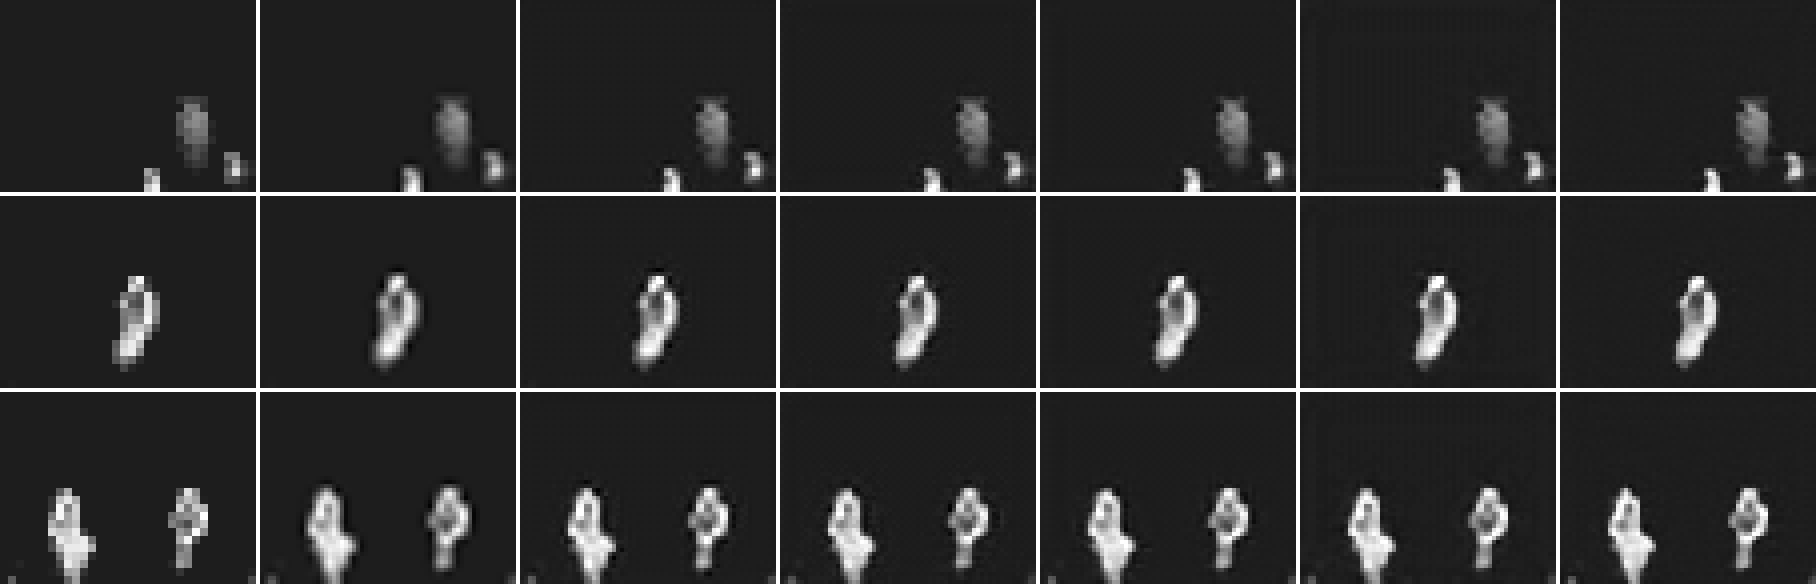
\includegraphics[width=\columnwidth]{qualitative_paper.png}
\caption{Native MLX90640 frames (32$\times$24) super-resolved on-device to
64$\times$48: LR input, bicubic, and the five INT8 models (qualitative --
no ground truth exists at the target resolution).}
\label{fig:qualitative}
\end{figure}

% TODO: bit-exactness note: on-board int8 outputs match the PC TFLite
% interpreter exactly (ref_mismatches = 0), so PC-side PSNR transfers
% verbatim to the deployed system.

\section{Conclusion}
% TODO

\bibliographystyle{IEEEtran}
\bibliography{refs}

\end{document}
